\chapter{RESIDUAL ATTENTION-BASED MYOCARDIAL SCAR SEGMENTATION AND QUANTIFICATION}

\label{chap:6}

\section{Overview}
\label{sec:ch6-intro-overview}

This chapter presents the final stage of the proposed deep learning framework for myocardial infarction assessment through residual attention-based myocardial scar segmentation and quantitative scar area assessment. Building upon the reliable anatomical myocardium representation established through the cardiac structure segmentation framework and loss function investigation presented in the previous chapters, this study focuses on identifying and quantifying myocardial scar tissue from multi-sequence cardiac magnetic resonance images to support objective myocardial infarction assessment.

Myocardial infarction (MI) causes irreversible myocardial injury that may subsequently lead to the formation of fibrotic scar tissue. The size and spatial distribution of myocardial scar are clinically relevant because they are associated with ventricular remodelling, impaired cardiac function, recurrent cardiac events, and patient prognosis. Therefore, accurate identification and quantitative assessment of myocardial scar constitute important components of CMR-based myocardial infarction analysis \citep{Richardson2015,Wu2021}.

Multi-sequence CMR provides complementary anatomical and pathological information by combining balanced Steady-State Free Precession (bSSFP), T2-weighted imaging (T2WI), and Late Gadolinium Enhancement (LGE). The bSSFP sequence primarily depicts cardiac anatomy, T2WI emphasizes myocardial oedema, whereas LGE provides high contrast for myocardial scar visualization. The spatial correspondence among these pre-aligned sequences enables complementary tissue characteristics to be jointly analysed, thereby providing a more comprehensive representation of myocardial pathology than any individual sequence alone \citep{Li2023MyoPS,Ding2023}.

Despite the availability of multi-sequence information, automated myocardial scar segmentation remains challenging. Scar regions are generally small, irregularly shaped, and heterogeneous in appearance. Their boundaries may also be difficult to distinguish from surrounding myocardial tissue. Conventional convolutional architectures may therefore fail to retain subtle pathological features or adequately emphasize the limited image regions associated with myocardial scar \citep{Wu2021}.

The investigations presented in Chapters IV and V established the anatomical foundation required for subsequent myocardial pathology analysis. Chapter IV developed an enhanced U-Net with fuzzy pooling for cardiac structure segmentation, whereas Chapter V investigated the influence of different loss functions on myocardium segmentation. Collectively, these investigations produced an improved myocardium representation that provides the anatomical basis for the myocardial scar analysis presented in this chapter.

To address the challenges associated with small, heterogeneous, and irregular myocardial scar regions, this chapter presents MyoScarNet-RA, a residual attention-based framework for myocardial scar segmentation and quantitative scar assessment. The proposed framework integrates residual learning and hybrid channel-spatial attention within a hierarchical encoder-decoder architecture. Residual connections facilitate effective information propagation through deep network layers, whereas the attention mechanism adaptively recalibrates channel and spatial feature responses to emphasize diagnostically relevant scar patterns while suppressing irrelevant background information \citep{He2016,Hu2018,Woo2018}.

The proposed framework does not terminate at pixel-wise segmentation. The predicted scar mask is further processed to estimate the physical scar area in square millimetres. This procedure enables segmentation output to be evaluated not only in terms of spatial correspondence with expert annotation but also through quantitative comparison between automated and manual scar area measurements \citep{Riandini2026Access}.

Accordingly, the objectives of this chapter are:

\begin{itemize}[nosep, leftmargin=*]
	\item to evaluate the capability of residual learning and hybrid attention for myocardial scar segmentation;
	\item to assess scar segmentation using overlap, boundary, and structural similarity measures;
	\item to estimate myocardial scar area from the predicted segmentation mask; and
	\item to evaluate the error, correlation, and agreement between automated scar area estimation and expert annotation.
\end{itemize}

The remainder of this chapter is organized as follows. Section~\ref{sec:ch6-framework} describes the proposed residual attention-based myocardial scar segmentation framework. Section~\ref{sec:ch6-materials} presents the dataset, image preparation, training configuration, reference architectures, and evaluation protocol. Section~\ref{sec:ch6-results} discusses the experimental results, including training behaviour, segmentation performance, scar area quantification, measurement agreement, and computational requirements. Section~\ref{sec:ch6-summary} summarizes the principal findings of the chapter.

\section{Proposed Residual Attention-Based Myocardial Scar Segmentation Framework}
\label{sec:ch6-framework}

The framework presented in this chapter extends the anatomical cardiac analysis established in Chapters IV and V toward automated myocardial scar segmentation and quantitative scar assessment. Rather than developing a completely independent segmentation pipeline, the proposed method builds upon the reliable myocardium representation obtained from the preceding investigations and focuses on identifying pathological scar tissue within multi-sequence CMR images. Using the proposed MyoScarNet-RA, the generated scar probability map is subsequently converted into a binary scar mask from which the physical scar area is estimated. Consequently, the framework integrates image segmentation and quantitative measurement into a unified analysis pipeline \citep{Riandini2026Access}.

\subsection{Overall Framework}
\label{subsec:ch6-overall}

The overall processing stages of the proposed framework are illustrated in Figure~\ref{fig:ch6-workflow}. The framework receives pre-aligned bSSFP, T2WI, and LGE images as complementary inputs. These images are prepared using the procedure described in Section~\ref{sec:ch6-materials} before being processed by the proposed residual attention network. The network generates a probability map representing the likelihood of scar presence at each pixel. The probability map is then converted into a binary scar mask, from which the scar area is calculated \citep{Li2023MyoPS,Riandini2026Access}.

\begin{figure}[htbp]
	\centering
	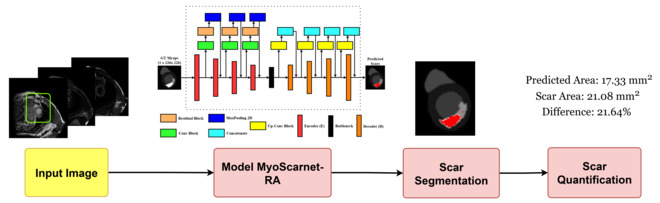
\includegraphics[width=\textwidth]{bab6/ch6-workflow.jpg}
	\caption{Overall workflow of the proposed myocardial scar segmentation and quantitative assessment framework \protect\citep{Riandini2026Access}}
	\label{fig:ch6-workflow}
\end{figure}

As shown in Figure~\ref{fig:ch6-workflow}, the framework consists of four sequential stages:

\begin{enumerate}[nosep, leftmargin=*]
	\item \textbf{Multi-sequence CMR input}, comprising spatially aligned bSSFP, T2WI, and LGE images.
	\item \textbf{Feature representation learning}, performed using residual blocks and hybrid channel-spatial attention.
	\item \textbf{Myocardial scar segmentation}, producing a pixel-wise scar probability map and binary scar mask.
	\item \textbf{Scar area quantification}, converting the segmented scar pixels into a physical area expressed in square millimetres.
\end{enumerate}

This sequential workflow establishes a direct dependency between scar segmentation and quantitative scar assessment. Since scar area estimation is computed directly from the segmented binary mask, inaccuracies in scar localization may propagate to the subsequent measurement stage. Consequently, reliable scar segmentation forms the computational foundation for accurate and reproducible myocardial scar quantification.

\subsection{MyoScarNet-RA Architecture}
\label{subsec:ch6-architecture}

MyoScarNet-RA is a single-stage hierarchical encoder-decoder network derived from the U-Net architecture for automated myocardial scar segmentation. The architecture integrates residual learning and hybrid channel-spatial attention to improve feature representation of small and heterogeneous scar regions while preserving efficient information propagation throughout the network. Residual blocks are incorporated throughout the encoder and decoder, whereas hybrid channel-spatial attention is applied at the bottleneck and after decoder feature fusion. The detailed architecture is shown in Figure~\ref{fig:ch6-architecture} \citep{Ronneberger2015,He2016,Riandini2026Access}.

\begin{figure}[htbp]
	\centering
	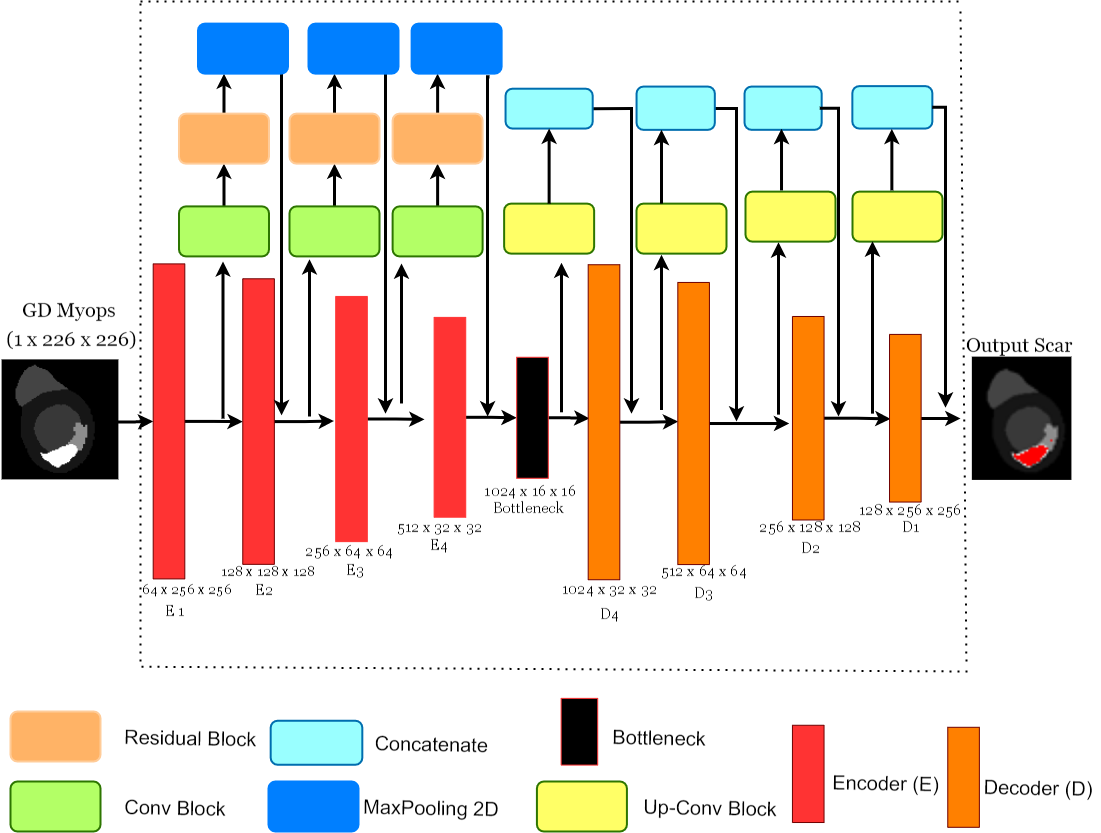
\includegraphics[width=\textwidth]{bab6/ch6-architecture.png}
	\caption{Architecture of the proposed MyoScarNet-RA for myocardial scar segmentation \protect\citep{Riandini2026Access}}
	\label{fig:ch6-architecture}
\end{figure}

As illustrated in Figure~\ref{fig:ch6-architecture}, feature extraction progresses through the encoder, information refinement is performed at the bottleneck using hybrid attention, and the decoder subsequently reconstructs the scar probability map through progressive feature fusion.

The architecture consists of three functional components:

\begin{itemize}[nosep, leftmargin=*]
	\item \textbf{Encoder}, responsible for extracting hierarchical image representations through four residual encoding stages;
	\item \textbf{Bottleneck}, responsible for refining the most abstract feature representation using residual learning and hybrid channel-spatial attention; and
	\item \textbf{Decoder}, responsible for reconstructing the final scar probability map through progressive feature fusion with skip connections.
\end{itemize}

The encoder consists of four stages, denoted as E1--E4. Each stage incorporates a residual block followed by max pooling. As the spatial resolution decreases, the number of feature channels increases, enabling the network to transform local intensity and texture information into more abstract representations of myocardial tissue and scar-related patterns. Residual connections are used to support information and gradient propagation through the deeper architecture \citep{He2016}.

At the bottleneck, a residual block is followed by hybrid channel-spatial attention. Channel attention assigns greater weight to feature channels containing relevant scar information, whereas spatial attention identifies image locations that are more likely to contain scar tissue. Their combination recalibrates the latent feature representation before spatial reconstruction begins \citep{Hu2018,Woo2018}.

The decoder comprises four stages, denoted as D4--D1. At each stage, the feature map is upsampled and concatenated with the corresponding encoder output. A residual block then refines the combined representation. Hybrid attention is applied following feature fusion so that the decoder can emphasize relevant scar characteristics at multiple spatial resolutions. A \(1 \times 1\)convolution followed by sigmoid activation produces the final probability map, with values ranging from zero to one \citep{Riandini2026Access}.

The complementary integration of residual learning and hybrid channel-spatial attention enables the proposed architecture to preserve efficient feature propagation while selectively emphasizing diagnostically relevant scar patterns. Consequently, the network learns both global contextual information and fine local scar characteristics, thereby improving feature representation of small and heterogeneous myocardial scar regions and supporting more accurate scar segmentation under complex myocardial tissue appearance \citep{He2016,Hu2018,Woo2018}.

The principal characteristics of MyoScarNet-RA can therefore be summarized as follows:

\begin{itemize}[nosep, leftmargin=*]
	\item
	residual blocks are used in both the encoder and decoder;
	\item
	hybrid channel-spatial attention is applied at the bottleneck and after decoder feature fusion;
	\item
	skip connections retain high-resolution spatial information;
	\item
	segmentation is completed in a single forward pass; and
	\item
	the network produces a pixel-wise scar probability map with an output resolution of $256 \times 256$ pixels.
\end{itemize}

\subsection{Myocardial Scar Segmentation}
\label{subsec:ch6-segmentation}

As illustrated in Figure~\ref{fig:ch6-architecture}, myocardial scar segmentation is performed through a single-stage encoder--decoder framework that transforms multi-sequence CMR images into a pixel-wise scar probability map. The three complementary CMR sequences are processed simultaneously to learn hierarchical feature representations describing both anatomical structures and pathological scar characteristics. These representations are progressively refined throughout the network before being reconstructed into the final segmentation output \citep{Riandini2026Access}.

During the forward propagation process, the encoder extracts increasingly abstract image features, while the bottleneck refines the latent representation through hybrid channel-spatial attention. The decoder subsequently restores spatial resolution by combining high-level semantic information with fine spatial features transferred through skip connections. This progressive reconstruction enables accurate localization of myocardial scar while preserving important anatomical details \citep{Ronneberger2015,Riandini2026Access}.

The final network output is a probability map, $P \in [0,1]^{H \times W}$, in which each pixel represents the estimated probability of belonging to the myocardial scar class. The probability map is subsequently converted into a binary scar mask using Otsu\textquotesingle s automatic thresholding procedure, as described in Section~\ref{subsec:ch6-area-method}. Because segmentation is completed within a single forward pass, the proposed framework does not require cascaded processing or an additional refinement network, thereby providing an efficient basis for subsequent quantitative scar area estimation \citep{Otsu1979,Riandini2026Access}.

\subsection{Myocardial Scar Area Quantification}
\label{subsec:ch6-area-method}

Following segmentation, the probability map produced by MyoScarNet-RA is converted into a binary scar mask using Otsu's automatic thresholding method. Otsu's method determines the threshold that maximizes the between-class variance of the pixel-value distribution, thereby separating scar and non-scar pixels without manual threshold selection \citep{Otsu1979}.

After thresholding, each non-zero pixel in the binary mask is interpreted as scar tissue. The total scar area is obtained by multiplying the number of scar pixels by the physical area represented by one pixel. This procedure is expressed as

\begin{equation}
	A_{\mathrm{scar}} = N_{\mathrm{scar}} \times R
	\label{eq:ch6-scar-area}
\end{equation}
where:
\begin{conditions}
	A_{\mathrm{scar}} & estimated myocardial scar area ($\text{mm}^2$); \\
	N_{\mathrm{scar}} & total number of non-zero pixels identified as scar tissue; and \\
	R & physical area represented by one image pixel ($\text{mm}^2/\text{pixel}$).
\end{conditions}

This formulation is consistent with the scar area quantification procedure implemented in Algorithm 2 of the source study, where scar size is calculated directly from the segmented binary mask \citep{Riandini2026Access}.

The complete quantification procedure adopted in this dissertation is summarized in Algorithm 6.1.

\begin{algorithm}[htbp]
	\caption{Automated Myocardial Scar Area Quantification}
	\label{alg:ch6-scar-quantification}
	\begin{algorithmic}[1]
		\Require Binary scar segmentation mask $M$, Pixel area $R$ ($\text{mm}^2$)
		\Ensure Estimated scar area $A_{\mathrm{scar}}$ ($\text{mm}^2$)
		\vspace{2pt}
		
		\State Convert the binary scar mask $M$ into a numerical array $M_{\mathrm{np}}$.
		\State Count the total number of scar pixels:
		\[
		N_{\mathrm{scar}} = \sum_{p \in M_{\mathrm{np}}} \mathbb{I}(p > 0)
		\]
		\Statex \hspace{\algorithmicindent} where $\mathbb{I}(\cdot)$ is the indicator function.
		\State Compute the scar area:
		\[
		A_{\mathrm{scar}} = N_{\mathrm{scar}} \times R
		\]
		\State \Return $A_{\mathrm{scar}}$
	\end{algorithmic}
\end{algorithm}

The estimated scar area is subsequently compared with the corresponding expert measurement. The quantitative evaluation includes absolute error, root mean square error, correlation analysis, and Bland--Altman agreement, which are presented in Section~\ref{sec:ch6-results}. The quantification procedure therefore provides a direct connection between the predicted scar mask and an interpretable physical measurement of scar extent.

\section{Materials and Experimental Setup}
\label{sec:ch6-materials}

The experiments presented in this chapter were conducted to evaluate the effectiveness of the proposed MyoScarNet-RA for myocardial scar segmentation and quantitative scar area estimation. To ensure a fair comparison, all evaluated models were implemented using identical dataset partitioning, preprocessing procedures, training configurations, and evaluation protocols. Consequently, any observed performance differences can be attributed primarily to architectural design rather than inconsistencies in the experimental protocol. The following subsections describe the dataset, image preparation, training configuration, and evaluation criteria adopted throughout the experimental study.

\subsection{MyoPS2020 Dataset}
\label{subsec:ch6-dataset}

The experiments were conducted using the \textbf{Myocardial Pathology Segmentation (MyoPS2020)} dataset, which contains pre-aligned multi-sequence CMR images together with expert annotations of myocardial pathology. Each subject includes three complementary imaging sequences, namely balanced Steady-State Free Precession (bSSFP), T2-weighted imaging (T2WI), and Late Gadolinium Enhancement (LGE). These three sequences provide complementary anatomical and pathological information that facilitates accurate myocardial scar segmentation \citep{Xue2020,Riandini2026Access}.

To avoid data leakage, dataset partitioning was performed at the patient level. Following the experimental protocol adopted in the source article, the dataset consisted of \textbf{36 patients for training (80\%)}, \textbf{5 patients for validation (11\%)}, and \textbf{4 patients for testing (9\%)}. This patient-wise partition ensures that images from the same subject are not simultaneously used for training and testing.




\begin{table}[h]
		\centering
		\caption{Dataset composition and patient-level splitting protocol} %\citep{Riandini2026Access}}
		\label{tab:ch6-partition}
		\begin{tabular}{lccc}
			\toprule
			\textbf{Set} & \textbf{Patients} & \textbf{Slices} & \textbf{Percentage} \\ \midrule
			Training     & 36                & 76              & 80\%       \\ 
			Validation   & 5                 & 15              & 11\%       \\ 
			Testing      & 4                 & 45              & 9\%        \\ \midrule
			\textbf{Total} & \textbf{45}     & \textbf{136}    & \textbf{100\%} \\ \bottomrule
		\end{tabular}
\end{table}
	


\begin{comment}
\begin{table}[htbp]
	\centering
	\fbox{\parbox{0.86\textwidth}{\centering Insert Patient-level dataset partition used throughout the experiments here}}
	\caption{Patient-level dataset partition used throughout the experiments \citep{Riandini2026Access}}
	\label{tab:ch6-partition}
\end{table}
%\noindent\textit{Source: Adapted from \citet{Riandini2026Access}.}
\end{comment}

The patient-wise data partition adopted in this study prevents images from the same subject from appearing in different subsets, thereby reducing the risk of information leakage during model development. This protocol enables a more reliable assessment of the proposed framework by ensuring that the reported performance reflects the ability of the network to generalize to previously unseen patients.

\subsection{Image Preparation and Training Configuration}
\label{subsec:ch6-preparation}

Image preparation followed the preprocessing procedure established in Chapter III to ensure methodological consistency throughout the dissertation. Briefly, all multi-sequence CMR images were resized to $256 \times 256$ pixels and subsequently normalized to reduce inter-image intensity variation. During training, data augmentation, including random horizontal flipping, image rotation, and image scaling, was applied to improve robustness against anatomical variability. The corresponding expert annotations were converted into binary scar masks and used as reference labels for supervised learning.

All experiments were implemented using the PyTorch deep learning framework under identical training settings for both the proposed model and the baseline architectures. A Dice-Cross Entropy loss function was applied during training using the Stochastic Gradient Descent (SGD) optimizer. The remaining implementation parameters, including batch size, learning-rate scheduling, and validation strategy, were maintained consistently throughout all experiments to ensure a fair comparison among the evaluated methods \citep{Riandini2026Access}.

\subsection{Reference Architectures and Evaluation Metrics}
\label{subsec:ch6-reference-models}

The effectiveness of the proposed MyoScarNet-RA was evaluated by comparison with two reference segmentation architectures, namely the \textbf{Simple U-Net} and the \textbf{Complex U-Net}. Both baseline models were trained using exactly the same dataset partition, preprocessing procedure, optimizer, and training configuration. Therefore, the comparative results reflect architectural differences rather than implementation bias.

Performance evaluation was conducted from both segmentation and quantitative assessment perspectives. Segmentation quality was assessed using the Dice Similarity Coefficient (DSC), Intersection over Union (IoU), Hausdorff Distance (HD), and Structural Similarity Index (SSIM). Quantitative scar estimation was subsequently evaluated using the Mean Absolute Error (MAE), Root Mean Square Error (RMSE), Pearson correlation coefficient, and Bland--Altman agreement analysis. Together, these complementary measurements provide a comprehensive evaluation of both segmentation accuracy and quantitative scar assessment capability \citep{Riandini2026Access}.

\section{Experimental Results and Discussion}
\label{sec:ch6-results}

\subsection{Training Behaviour Analysis}
\label{subsec:ch6-training}

The training behaviour of the proposed MyoScarNet-RA was first analysed to evaluate the convergence characteristics of the learning process before quantitative segmentation performance was assessed. Throughout training, both the training and validation datasets were monitored to examine whether the network learned representative myocardial scar features while maintaining stable generalization.

Figure~\ref{fig:ch6-training} illustrates the evolution of training accuracy and loss during the learning process.

\begin{figure}[htbp]
	\centering
	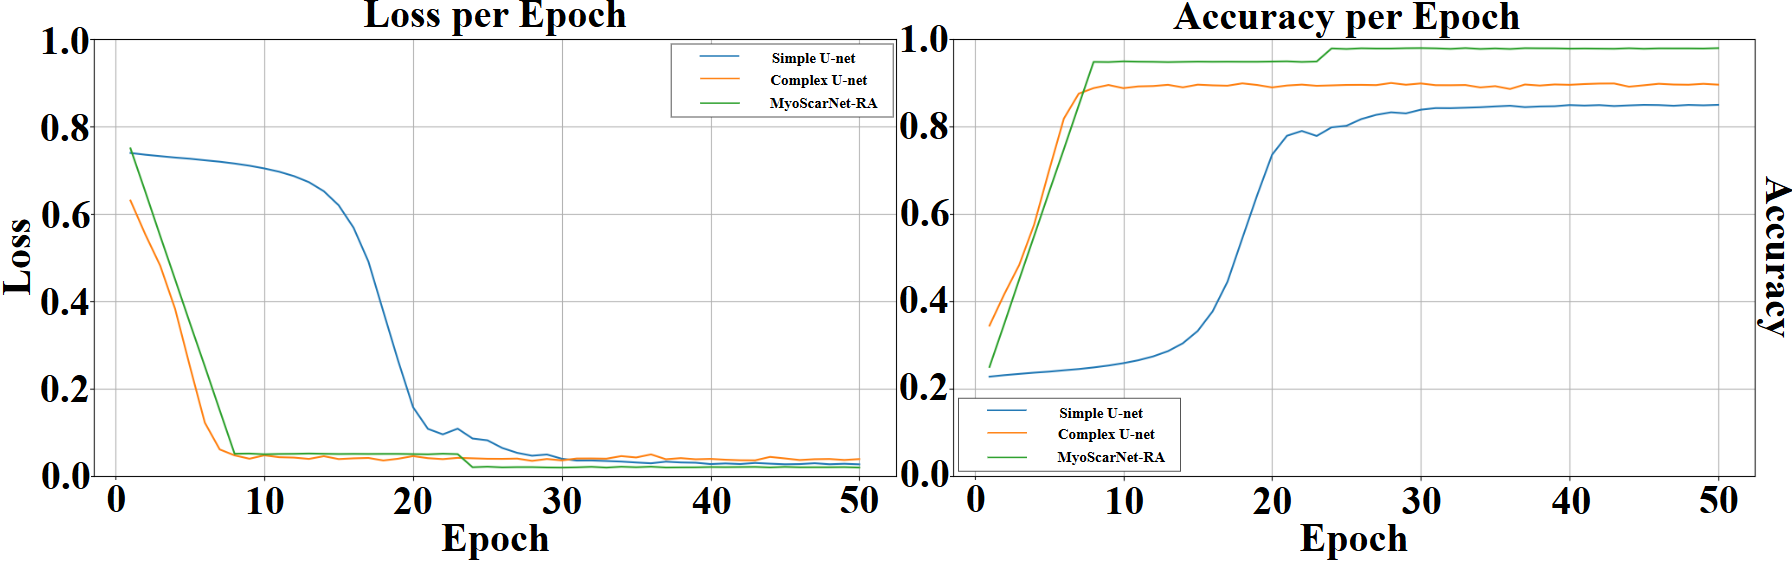
\includegraphics[width=\textwidth]{bab6/ch6-training.png}
	\caption{Training accuracy and loss curves of the proposed MyoScarNet-RA \protect\citep{Riandini2026Access}}
	\label{fig:ch6-training}
\end{figure}

\begin{comment}
\begin{figure}[htbp]
	\centering
	\fbox{\parbox{0.86\textwidth}{\centering Insert Training accuracy and loss curves of the proposed MyoScarNet-RA here}}
	\caption{Training accuracy and loss curves of the proposed MyoScarNet-RA \citep{Riandini2026Access}}
	\label{fig:ch6-training}
\end{figure}
%\noindent\textit{Source: Adapted from \citet{Riandini2026Access}.}
\end{comment}

As illustrated in Figure~\ref{fig:ch6-training}, the training accuracy increased progressively throughout the learning process, accompanied by a consistent reduction in both the training and validation losses. The similar trends exhibited by the two loss curves indicate that the proposed MyoScarNet-RA achieved stable learning behaviour without noticeable divergence between training and validation performance. This behaviour suggests that the network successfully learned representative myocardial scar features while maintaining satisfactory generalization to previously unseen validation samples.

Overall, the learning behaviour observed in Figure~\ref{fig:ch6-training} demonstrates that the adopted training configuration enabled stable model convergence before quantitative evaluation was performed. Establishing stable learning behaviour is important because the segmentation results presented in the following subsection should reflect the effectiveness of the proposed residual attention architecture rather than instability during network training.

\subsection{Scar Segmentation Performance}
\label{subsec:ch6-performance}

The segmentation performance of the proposed MyoScarNet-RA was quantitatively evaluated by comparison with the reference segmentation architectures under identical experimental conditions. The comparison employed four complementary performance measures, namely the Dice Similarity Coefficient (DSC), Intersection over Union (IoU), Hausdorff Distance (HD), and Structural Similarity Index (SSIM). Collectively, these metrics evaluate regional overlap, boundary accuracy, and structural similarity between the predicted scar segmentation and the corresponding expert annotation.

The quantitative comparison is presented in Table~\ref{tab:ch6-segmentation}, whereas representative segmentation examples are illustrated in Figure~\ref{fig:ch6-segmentation}.

\subsection{Scar Segmentation Performance}
\label{subsec:ch6-performance}

The segmentation performance of the proposed MyoScarNet-RA was quantitatively evaluated by comparison with the reference segmentation architectures under identical experimental conditions. The comparison employed six complementary performance measures, namely the Dice Similarity Coefficient (DSC), Intersection over Union (IoU), Hausdorff Distance (HD), Structural Similarity Index (SSIM), Sensitivity (SEN), and Specificity (SPE). Collectively, these metrics evaluate regional overlap, boundary accuracy, structural similarity, and voxel classification quality between the predicted scar segmentation and the corresponding expert annotation.

The quantitative comparison is presented in Table~\ref{tab:performance_comparison}, whereas representative segmentation examples are illustrated in Figure~\ref{fig:ch6-segmentation}.

\begin{table}[htbp]
	\centering
	\caption{Quantitative comparison of myocardial scar segmentation performance}
	\label{tab:performance_comparison}
	
	\small
	\setlength{\heavyrulewidth}{\lightrulewidth}
	\renewcommand{\arraystretch}{1.25} % Memberi ruang vertikal agar tidak terlalu rapat
	
	\begin{tabularx}{\textwidth}{
			>{\raggedright\arraybackslash}p{0.30\textwidth}
			>{\centering\arraybackslash}X
			>{\centering\arraybackslash}X
			>{\centering\arraybackslash}X
		}
		\toprule
		\textbf{Metric} & \textbf{Simple U-Net} & \textbf{Complex U-Net} & \textbf{MyoScarNet-RA} \\
		\midrule
		Residual (\cmark/\xmark) & \xmark & \cmark & \cmark \\
		Attention (\cmark/\xmark) & \xmark & \xmark & \cmark \\
		\midrule
		IoU & $0.8301 \pm 0.0875$ & $\mathbf{0.8880 \pm 0.0496}$ & $0.8758 \pm 0.0625$ \\
		HD (mm) & $11.45 \pm 10.44$ & $2.43 \pm 4.01$ & $\mathbf{1.31 \pm 0.53}$ \\
		Dice Score & $0.9047 \pm 0.0526$ & $0.9071 \pm 0.0279$ & $\mathbf{0.9326 \pm 0.0368}$ \\
		SSIM & $0.9132 \pm 0.0474$ & $\mathbf{0.9466 \pm 0.0241}$ & $0.9406 \pm 0.0301$ \\
		Sensitivity (SEN) & $\mathbf{0.9980 \pm 0.0025}$ & $0.9960 \pm 0.0065$ & $0.9795 \pm 0.0210$ \\
		Specificity (SPE) & $0.9992 \pm 0.0005$ & $0.9995 \pm 0.0003$ & $\mathbf{0.9996 \pm 0.0002}$ \\
		\bottomrule
		\multicolumn{4}{@{}p{\textwidth}@{}}{\vspace{4pt}\footnotesize 
			$^{\dagger}$ Values are reported as Mean $\pm$ SD evaluated on the MyoPS2020 dataset. \newline
			$^*$ HD = Hausdorff Distance; SSIM = Structural Similarity Index; SEN = Sensitivity; SPE = Specificity. Checkmarks (\cmark) indicate presence of architectural component; crosses (\xmark) indicate absence. Bold text indicates the best performance for each metric. \newline
			\textit{Source:} Adapted from \citet{Riandini2026Access}.}
	\end{tabularx}
\end{table}

\begin{comment}
\begin{table}[htbp]
	\centering
	\fbox{\parbox{0.86\textwidth}{\centering Insert quantitative comparison of myocardial scar segmentation performance here}}
	\caption{Quantitative comparison of myocardial scar segmentation performance \citep{Riandini2026Access}}
	\label{tab:ch6-segmentation}
\end{table}
%\noindent\textit{Source: Adapted from \citet{Riandini2026Access}.}
\end{comment}

As summarized in Table~\ref{tab:performance_comparison}, the proposed MyoScarNet-RA demonstrated highly competitive segmentation performance across all evaluated metrics. Although the Complex U-Net achieved the highest IoU ($0.8880 \pm 0.0496$) and SSIM ($0.9466 \pm 0.0241$), the proposed MyoScarNet-RA demonstrated the highest Dice score ($0.9326 \pm 0.0368$) and the best Hausdorff Distance ($1.3117 \pm 0.5287~\text{mm}$), indicating superior boundary localization accuracy. Furthermore, all evaluated models exhibited excellent specificity ($>0.999$) and high sensitivity ($>0.97$), confirming consistent background suppression and reliable scar identification across multi-sequence CMR images.


\begin{figure}[htbp]
	\centering
	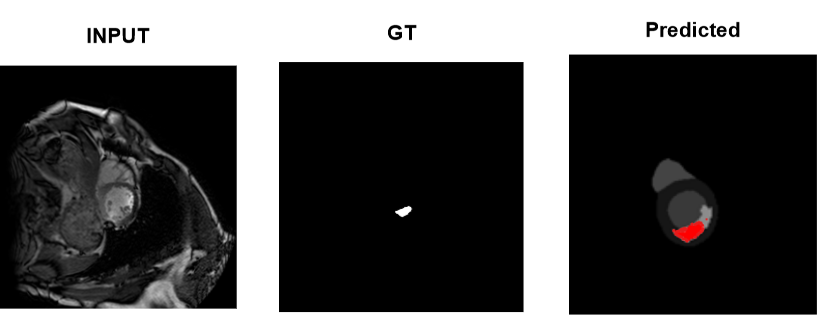
\includegraphics[width=\textwidth]{bab6/ch6-segmentation.png}
	\caption{Example of myocardial scar segmentation result obtained using the proposed MyoScarNet-RA \protect\citep{Riandini2026Access}}
	\label{fig:ch6-segmentation}
\end{figure}

The qualitative comparison presented in Figure~\ref{fig:ch6-segmentation} is consistent with these quantitative results. Relative to the Simple U-Net and Complex U-Net, the segmentation generated by MyoScarNet-RA follows the reference scar regions more consistently while reducing fragmented predictions and irregular boundary discontinuities. The improvement is particularly apparent in slices containing small and heterogeneous scar regions, where accurate localization is generally more challenging because of subtle intensity variation across the infarcted myocardium.

The observed segmentation performance can be attributed to the complementary interaction between residual learning and hybrid channel-spatial attention. Residual connections facilitate effective feature propagation throughout the network, whereas the attention mechanism selectively enhances diagnostically relevant scar features while suppressing irrelevant background responses. Consequently, the proposed architecture preserves both global contextual information and local scar characteristics, contributing to accurate boundary localization and reliable myocardial scar segmentation.


\subsection{Scar Area Quantification}
\label{subsec:ch6-area-results}

Following the evaluation of scar segmentation performance, the subsequent analysis investigates whether the generated segmentation masks can provide reliable quantitative scar measurements. Since the primary objective of the proposed framework is not only to identify scar tissue but also to estimate its physical extent, quantitative agreement between the automatically estimated scar area and the corresponding reference measurement becomes an essential indicator of the practical applicability of the proposed method.

The quantitative performance of the proposed scar area estimation was evaluated using the Mean Absolute Error (MAE), Root Mean Square Error (RMSE), and Pearson Correlation Coefficient (r). These complementary metrics respectively quantify the average estimation error, the magnitude of prediction deviation, and the degree of linear agreement between the automatically estimated scar area and the corresponding manual measurements performed by expert clinicians.

The evaluation metrics are formulated as follows:

\begin{equation}
	\mathrm{MAE}=\frac{1}{n}\sum_{i=1}^{n}\left|\hat{A}_{i}-A_{i}\right|
	\label{eq:ch6-mae}
\end{equation}

\begin{equation}
	\mathrm{RMSE}=\sqrt{\frac{1}{n}\sum_{i=1}^{n}\left(\hat{A}_{i}-A_{i}\right)^2}
	\label{eq:ch6-rmse}
\end{equation}

\begin{equation}
	r=\frac{\sum_{i=1}^{n}(\hat{A}_{i}-\overline{\hat{A}})(A_{i}-\overline{A})}{\sqrt{\sum_{i=1}^{n}(\hat{A}_{i}-\overline{\hat{A}})^2}\sqrt{\sum_{i=1}^{n}(A_{i}-\overline{A})^2}}
	\label{eq:ch6-pcc}
\end{equation}

where $\hat{A}_{i}$ and $A_i$ denote the automated and reference scar-area measurements for sample $i$, respectively, and $n$ is the number of evaluated samples.

The quantitative comparison between automated scar area estimation and manual measurement is summarized in Table~\ref{tab:ch6-area}. The proposed framework produced low estimation errors together with a strong linear relationship between the automatically estimated scar area and the corresponding expert measurements. These findings demonstrate that the proposed framework is capable of providing reliable scar area estimation, thereby providing a solid foundation for the agreement analysis presented in Section~\ref{subsec:ch6-agreement}.

\begin{comment}
	\begin{table}[htbp]
		\centering
		\fbox{\parbox{0.86\textwidth}{\centering Insert Quantitative evaluation of myocardial scar area estimation here}}
		\caption{Quantitative evaluation of myocardial scar area estimation \citep{Riandini2026Access}}
		\label{tab:ch6-area}
	\end{table}
	%\noindent\textit{Source: Adapted from \citet{Riandini2026Access}.}
\end{comment}

\begin{table}[htbp]
	\centering
	\caption{Scar area quantification: automated vs. manual annotation (our test split) \citep{Riandini2026Access}}
	\label{tab:ch6-area}
	
	\small
	\resizebox{\linewidth}{!}{%
		\begin{tabular}{lccc}
			\toprule
			\textbf{Image ID} & \textbf{Automated (mm$^2$)} & \textbf{Manual GT (mm$^2$)} & \textbf{Error (mm$^2$)} \\ \midrule
			117\_slice\_3 & 54.69 & 45.52 & +9.17 \\
			112\_slice\_3 & 29.00 & 24.16 & +4.84 \\
			107\_slice\_2 & 78.44 & 69.38 & +9.06 \\
			104\_slice\_0 & 65.69 & 52.60 & +13.09 \\
			120\_slice\_1 & 35.94 & 33.75 & +2.19 \\
			112\_slice\_0 & 16.62 & 16.77 & -0.15 \\
			119\_slice\_3 & 61.50 & 58.46 & +3.04 \\
			109\_slice\_0 & 20.06 & 16.46 & +3.60 \\
			121\_slice\_1 & 56.06 & 43.66 & +12.40 \\
			101\_slice\_3 & 48.62 & 41.04 & +7.58 \\
			103\_slice\_1 & 15.06 & 11.18 & +3.88 \\
			113\_slice\_0 & 26.00 & 20.56 & +5.44 \\
			116\_slice\_2 & 45.31 & 44.11 & +1.20 \\
			109\_slice\_1 & 41.56 & 35.37 & +6.19 \\
			122\_slice\_3 & 76.94 & 66.49 & +10.45 \\
			124\_slice\_2 & 52.44 & 46.49 & +5.95 \\ \bottomrule
		\end{tabular}%
	}
	
	\vspace{2mm}
	\begin{minipage}{\linewidth}
		\footnotesize
		\noindent $*$ Values are computed using our preprocessing and patient-level split; absolute errors can vary under different annotation protocols, slice selection rules, and data partitions.
	\end{minipage}
\end{table}

The representative examples presented in Figure~\ref{fig:ch6-area} visually demonstrate the capability of the proposed framework to estimate myocardial scar area across different infarction patterns. Despite variations in scar morphology, size, and spatial distribution, the estimated scar regions closely correspond to the manually annotated reference, indicating consistent preservation of scar extent and location. These visual observations are consistent with the quantitative results summarized in Table~\ref{tab:ch6-area} and further support the reliability of the proposed scar area estimation.

\begin{figure}[htbp]
	\centering
	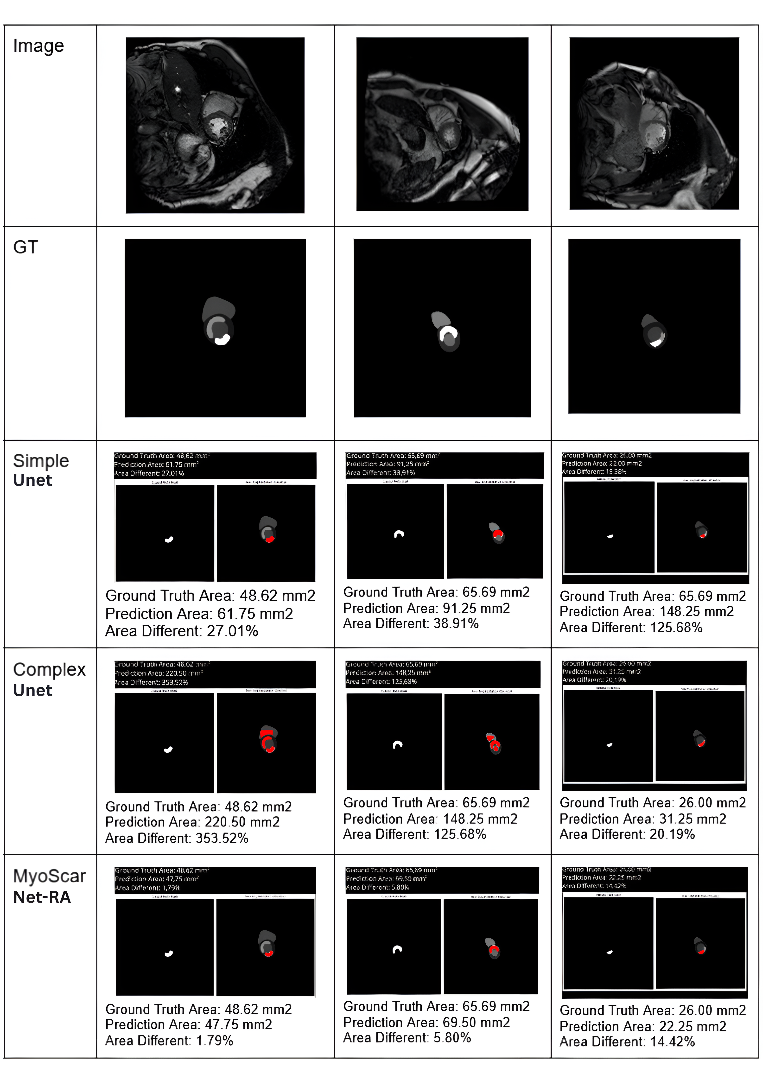
\includegraphics[width=\textwidth]{bab6/ch6-area.png}
	\caption{Representative examples of myocardial scar area estimation obtained using the proposed MyoScarNet-RA \protect\citep{Riandini2026Access}}
	\label{fig:ch6-area}
\end{figure}

The favourable quantitative performance observed in this study reflects the close relationship between scar segmentation accuracy and subsequent scar area estimation. Because scar area is calculated directly from the segmented scar mask, improvements in segmentation accuracy and reduction of boundary errors are translated into more reliable quantitative measurements. These findings indicate that accurate scar segmentation serves as the computational foundation for objective scar area estimation throughout the proposed framework.

Taken together, the quantitative results presented in Table~\ref{tab:ch6-area} and the representative examples shown in Figure~\ref{fig:ch6-area} demonstrate that accurate scar segmentation can be consistently translated into reliable physical scar area estimation, providing an objective representation of myocardial scar extent that complements conventional visual image interpretation.

From a clinical perspective, scar area quantification provides complementary information beyond visual interpretation alone. Rather than relying solely on qualitative visual assessment, clinicians are provided with an objective estimate of infarct extent that may support treatment planning, longitudinal patient follow-up, and evaluation of myocardial injury severity.

\subsection{Agreement Analysis}
\label{subsec:ch6-agreement}

Although the correlation analysis presented in the previous subsection demonstrates a strong linear relationship between automated and manual scar area measurements, correlation alone does not indicate whether the two measurement methods agree sufficiently for quantitative assessment. Therefore, Bland--Altman analysis was performed to evaluate the measurement agreement by analysing the distribution of estimation errors and identifying the presence of systematic measurement bias.

For each sample, the mean and difference between the automated and reference measurements are calculated as:
\begin{align}
	M_i &= \frac{\hat{A}_i + A_i}{2} \label{eq:ch6-ba-mean} \\
	D_i &= \hat{A}_i - A_i \label{eq:ch6-ba-difference}
\end{align}

The mean bias is:
\begin{equation}
	\overline{D} = \frac{1}{n} \sum_{i=1}^{n} D_i
	\label{eq:ch6-ba-bias}
\end{equation}

and the upper and lower 95\% limits of agreement are:
\begin{align}
	\mathrm{LoA}_{\mathrm{upper}} &= \overline{D} + 1.96 s_D \label{eq:ch6-ba-upper} \\
	\mathrm{LoA}_{\mathrm{lower}} &= \overline{D} - 1.96 s_D \label{eq:ch6-ba-lower}
\end{align}
where $s_D$ denotes the standard deviation of the measurement differences.

The agreement between automated and manual scar area measurements is illustrated in Figure~\ref{fig:ch6-bland-altman}.

\begin{comment}
\begin{figure}[htbp]
	\centering
	\fbox{\parbox{0.86\textwidth}{\centering Insert Bland--Altman plot comparing automated myocardial scar area estimation with expert measurements here}}
	\caption{Bland--Altman plot comparing automated myocardial scar area estimation with expert measurements \citep{Riandini2026Access}}
	\label{fig:ch6-bland-altman}
\end{figure}
%\noindent\textit{Source: Adapted from \citet{Riandini2026Access}.}
\end{comment}

\begin{figure}[htbp]
	\centering
	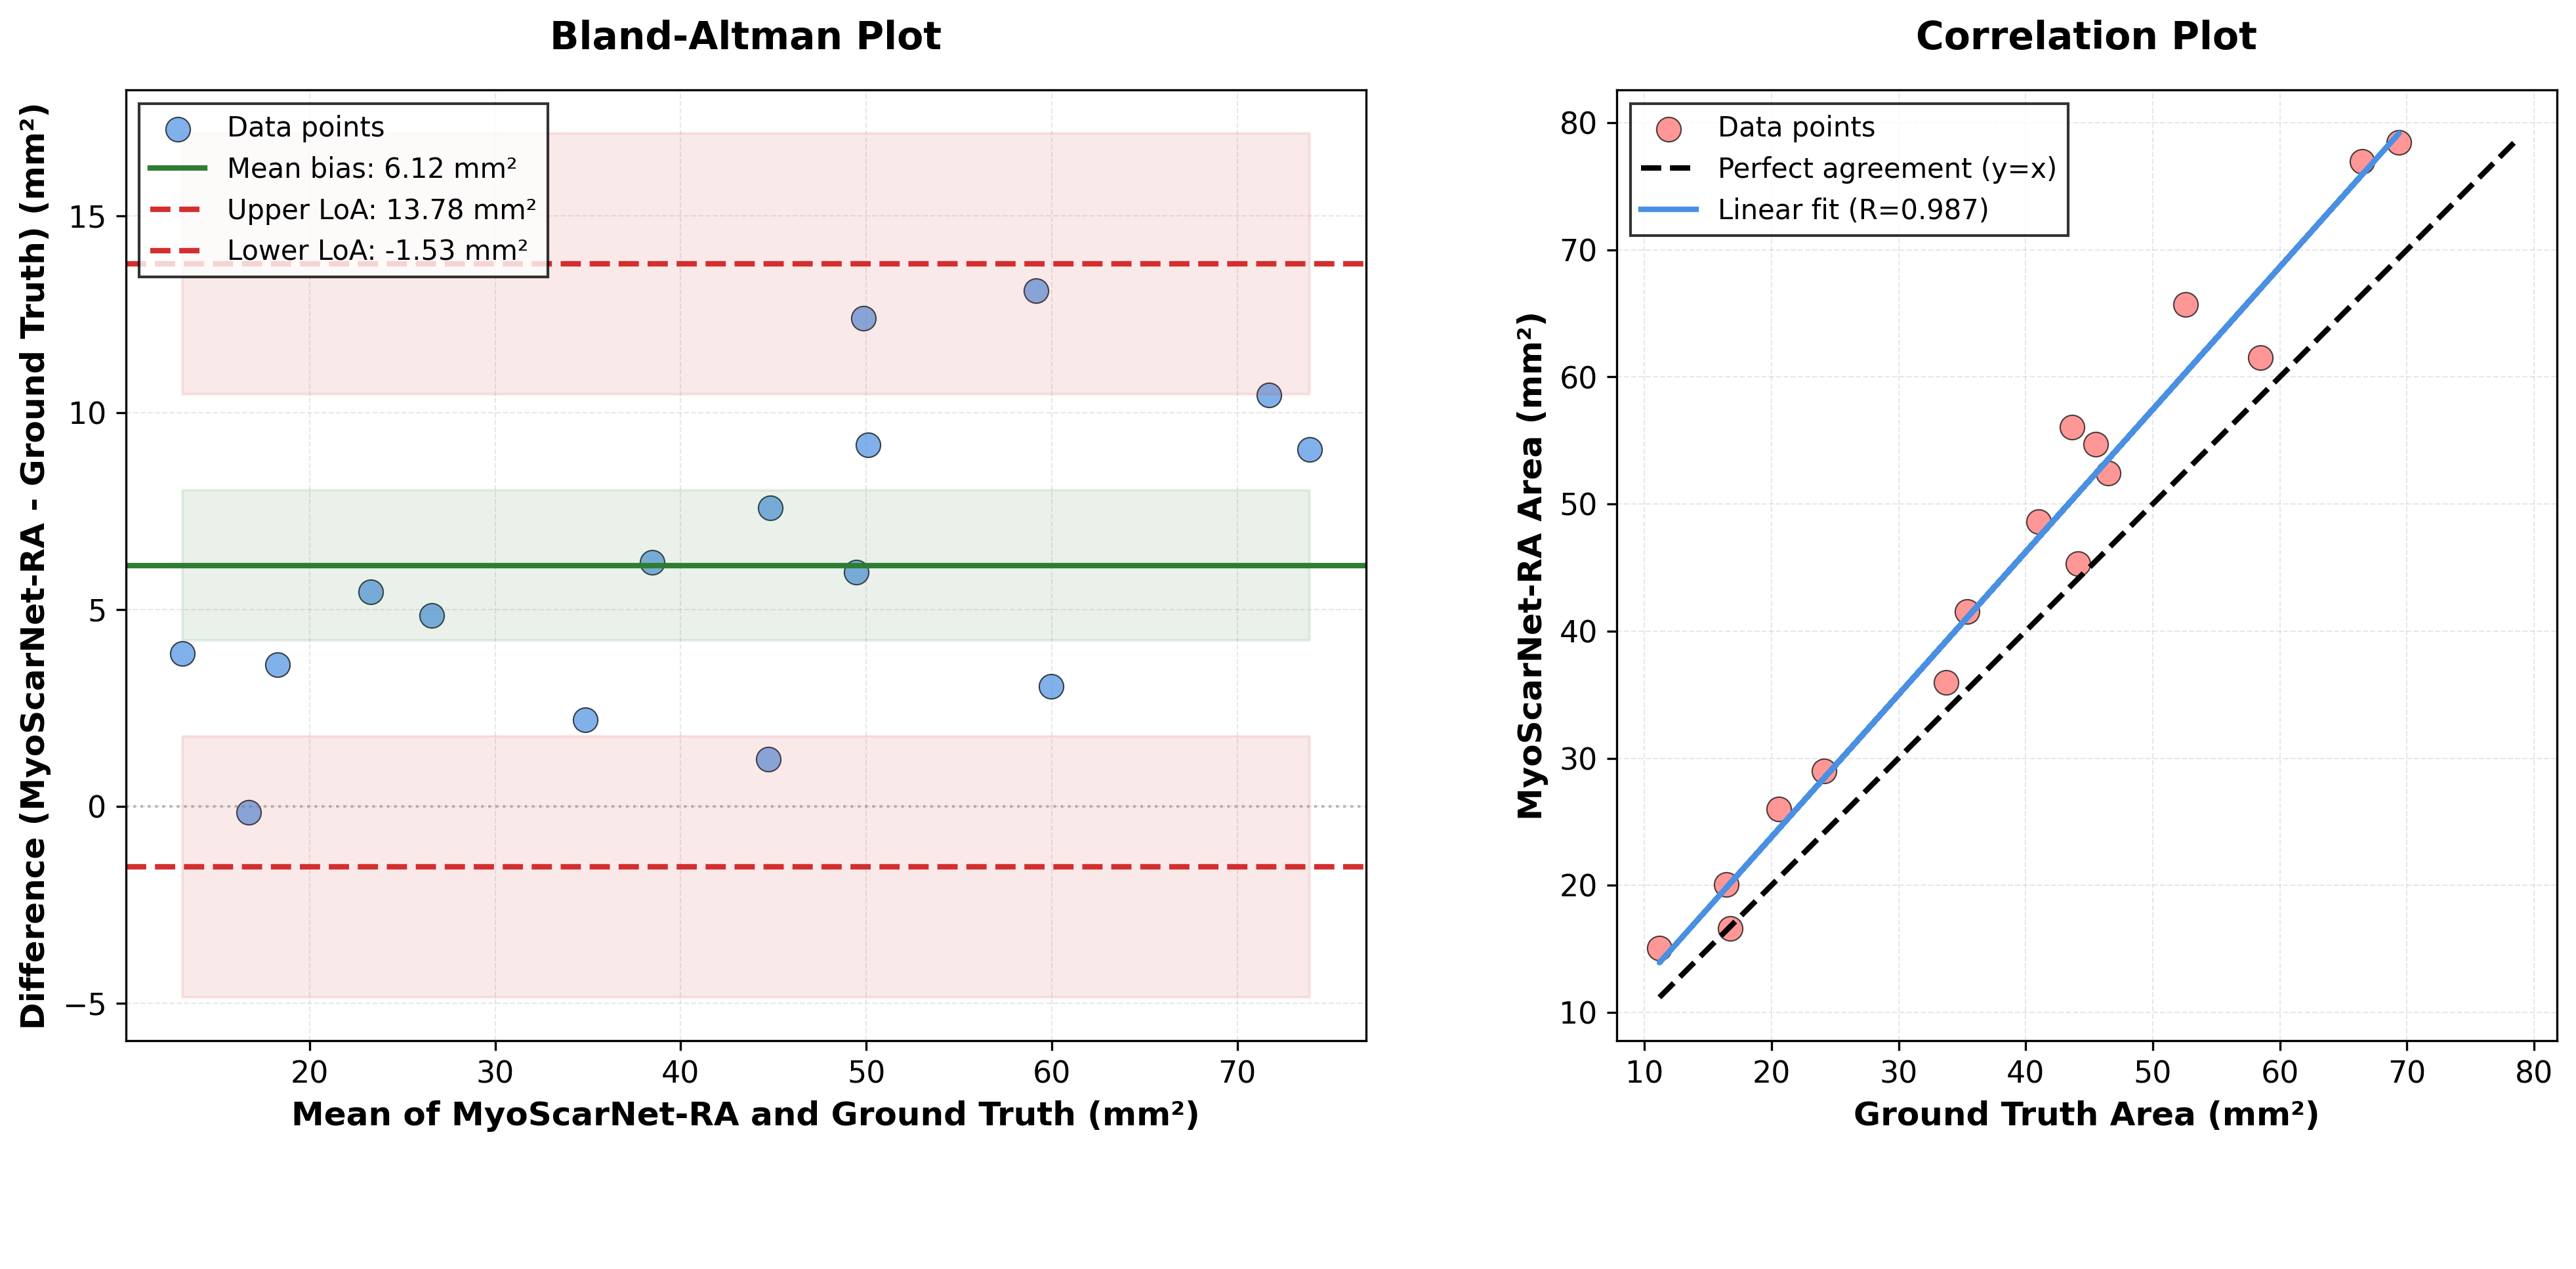
\includegraphics[width=\textwidth]{bab6/ch6-bland-altman.png}
	\caption{Bland--Altman plot analysis comparing automated myocardial scar area estimation with expert/manual measurements \protect\citep{Riandini2026Access}}
	\label{fig:ch6-bland-altman}
\end{figure}

As presented in Figure~\ref{fig:ch6-bland-altman}, the majority of measurement differences are distributed within the 95\% limits of agreement, indicating satisfactory agreement between the automated scar area estimation and the corresponding manual measurements. Only a limited number of observations are located near the agreement boundaries, suggesting that substantial estimation errors occur infrequently across the evaluated dataset.

The Bland--Altman analysis complements the correlation analysis presented in the previous subsection. While the Pearson correlation coefficient confirmed a strong linear relationship between automated and manual measurements, the Bland--Altman plot demonstrates that the differences between the two measurement methods remained relatively small and were randomly distributed around the mean bias. Together, these findings indicate that the proposed framework provides both a strong linear association and satisfactory agreement with expert measurements. These complementary agreement analyses demonstrate that the proposed scar quantification framework is capable of producing consistent quantitative measurements across the evaluated dataset.

From a clinical perspective, reliable measurement agreement is particularly important because myocardial scar area may influence patient risk stratification and treatment planning. The relatively small measurement bias obtained in this study suggests that the proposed framework can provide consistent quantitative scar estimation while maintaining close agreement with manual measurements performed by experienced observers. Consequently, the automated quantification procedure has the potential to reduce measurement variability and improve reproducibility without replacing expert clinical judgement.

\subsection{Computational Performance Analysis}
\label{subsec:ch6-computation}

In addition to segmentation accuracy and quantitative scar assessment, the computational characteristics of the proposed framework were also evaluated to determine its practical feasibility. Besides achieving high segmentation performance, a computer-aided myocardial scar analysis system should maintain computational requirements that remain compatible with routine deep learning implementation. Therefore, computational performance was assessed by considering both model complexity and inference efficiency.

The computational comparison between the proposed MyoScarNet-RA and the reference architectures is summarized in Table~\ref{tab:ch6-computation}.

\begin{table}[htbp]
	\centering
	\caption{Computational performance comparison of the evaluated segmentation frameworks}% \citep{Riandini2026Access}}
	\label{tab:ch6-computation}
	
	\small
	\resizebox{\linewidth}{!}{%
		\begin{tabular}{lccc}
			\toprule
			\textbf{Model} & \textbf{Avg. Time/Epoch (s)} & \textbf{Params} & \textbf{GPU Mem (GB)} \\ \midrule
			Simple U-Net   & $\mathbf{0.3684}$            & 7.76M           & 3.89                  \\
			Complex U-Net  & 1.5188                       & 31.04M          & 0.61                  \\
			\textbf{MyoScarNet-RA} & 2.1556                & 34.15M          & $\mathbf{0.40}$       \\ \midrule
			\textbf{Average:} & 1.3476                    & 18.30M          & 1.6367                \\ \bottomrule
		\end{tabular}%
	}
\end{table}

\begin{comment}
	\begin{table}[htbp]
		\centering
		\fbox{\parbox{0.86\textwidth}{\centering Insert computational performance comparison of the evaluated segmentation frameworks here}}
		\caption{Computational performance comparison of the evaluated segmentation frameworks \citep{Riandini2026Access}}
		\label{tab:ch6-computation}
	\end{table}
	%\noindent\textit{Source: Adapted from \citet{Riandini2026Access}.}
\end{comment}

As presented in Table~\ref{tab:ch6-computation}, incorporating residual learning and hybrid channel-spatial attention inevitably increased the architectural complexity compared with the conventional U-Net variants. Nevertheless, the proposed MyoScarNet-RA achieves the lowest GPU memory usage ($0.40~\text{GB}$) despite higher parameter count ($34.15\text{M}$) and computational time ($2.1556~\text{s/epoch}$), indicating efficiency in memory management while maintaining performance. These findings indicate that the additional computational cost is justified by the corresponding gain in analytical performance, resulting in a favourable balance between model complexity and segmentation capability.

Despite the inclusion of additional residual and attention modules, the proposed architecture maintained computational requirements that are compatible with contemporary GPU-based deep learning systems. This observation indicates that the improved segmentation performance was achieved without imposing excessive computational burden, thereby supporting the practical applicability of the proposed framework for automated myocardial scar analysis.

From the perspective of clinical implementation, computational efficiency is an important consideration because automated analysis should provide results within a reasonable processing time while maintaining high segmentation accuracy. The computational characteristics observed in this study demonstrate that the proposed MyoScarNet-RA satisfies these practical requirements by providing improved myocardial scar segmentation together with acceptable computational complexity.

\subsection{Overall Discussion}
\label{subsec:ch6-discussion}

The experimental results collectively demonstrate that the proposed MyoScarNet-RA provides a coherent framework for integrating myocardial scar segmentation with quantitative scar area estimation. The stable learning behaviour observed during training, together with the competitive segmentation performance and satisfactory quantitative agreement with expert measurements, indicates that the proposed architecture successfully preserves diagnostically relevant scar features throughout the complete analysis pipeline. Rather than evaluating segmentation and quantification as independent tasks, the present study demonstrates that accurate scar segmentation forms the computational basis for reliable quantitative scar assessment.

The complementary use of segmentation metrics, quantitative error measurements, correlation analysis, and Bland--Altman agreement provides a comprehensive evaluation of the proposed framework from multiple perspectives. Rather than relying on a single performance indicator, these analyses collectively demonstrate that the predicted scar masks preserve sufficient anatomical information for subsequent quantitative assessment. Consequently, the proposed framework extends conventional image segmentation toward objective myocardial scar quantification that may assist clinical interpretation.

Despite these encouraging findings, several limitations should be acknowledged. The proposed framework was evaluated using the MyoPS2020 dataset, and its generalization to larger multi-centre datasets remains to be investigated. In addition, the present study focused exclusively on myocardial scar segmentation and scar area quantification without incorporating clinical outcome prediction or prognostic analysis. These aspects provide opportunities for future research aimed at extending the applicability of the proposed framework while preserving the anatomical foundation established throughout this dissertation.

Overall, this chapter demonstrates that the proposed MyoScarNet-RA effectively extends anatomical myocardium segmentation toward automated myocardial scar segmentation and quantitative scar assessment. Together with the investigations presented in Chapters IV and V, the present study establishes a coherent deep learning-based framework for CMR image analysis, beginning with anatomical cardiac structure segmentation, followed by improved myocardium segmentation through loss function investigation, and culminating in automated myocardial scar segmentation and quantitative scar assessment. Collectively, these contributions establish an integrated framework for objective myocardial infarction analysis using CMR.

\section{Chapter Summary}
\label{sec:ch6-summary}

This chapter presented MyoScarNet-RA, a residual attention-based framework for automated myocardial scar segmentation and quantitative scar area assessment using multi-sequence CMR images. Building upon the reliable myocardium segmentation established in Chapter V, the proposed framework enabled accurate myocardial scar segmentation and scar area estimation.

Experimental results demonstrated that the proposed framework supports CMR-based myocardial scar assessment. Together with the investigations presented in Chapters IV and V, this chapter completes the proposed deep learning framework developed in this dissertation. The following chapter presents the overall conclusions, scientific contributions, study limitations, and future research directions.
